% The commuting triangle behind inclusion reversal: the Artin map of
% M/K composed with restriction gives the Artin map of L/K.
% Source: book/tex/alg-NT/artin.tex (§ Artin reciprocity,
% inclusion-reversing lemma) — tikzcd.
\documentclass[border=2mm]{standalone}
\usepackage{tikz}
\usetikzlibrary{arrows.meta}
\usepackage{amssymb}
\usepackage{amsmath}
\begin{document}
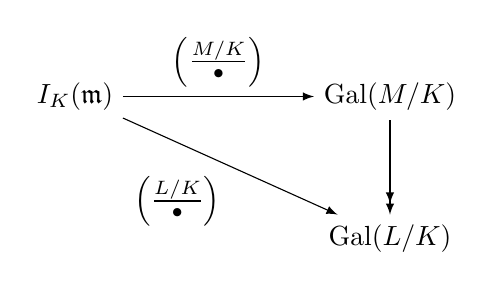
\begin{tikzpicture}[>=latex]
  \node (I) at (0,1.8) {$I_K(\mathfrak{m})$};
  \node (M) at (4,1.8) {$\operatorname{Gal}(M/K)$};
  \node (L) at (4,0) {$\operatorname{Gal}(L/K)$};
  \draw[->] (I) -- (M) node[midway,above] {$\left( \frac{M/K}{\bullet} \right)$};
  \draw[->] (I) -- (L) node[midway,below left] {$\left( \frac{L/K}{\bullet} \right)$};
  \draw[->>] (M) -- (L);
\end{tikzpicture}
\end{document}
